\documentclass[final]{beamer}

\usepackage[size=custom,width=100,height=100,orientation=landscape]{beamerposter}

\mode<presentation>{\usetheme{CoEPPoster}}

\usepackage[english]{babel}
\usepackage[T1]{fontenc}
\usepackage{amsmath,amsthm, amssymb, latexsym}
\usepackage[disable]{todonotes} 
\usepackage{array,booktabs,tabularx,enumitem}

\newcolumntype{Z}{>{\centering\arraybackslash}X} % centered tabularx columns
\newcommand{\comment}[1]{}
\newcommand{\generic}[7]{\ensuremath{#1{\bf \mathcal{#2}}_{#3}^{#4,#5} [\{#6\} (#7)]}}

\addtobeamertemplate{block end}{}{\vspace*{2ex}} % White space under blocks
\addtobeamertemplate{block alerted end}{}{\vspace*{2ex}} % White space under highlighted (alert) blocks

\setlength{\belowcaptionskip}{2ex} % White space under figures
\setlength\belowdisplayshortskip{2ex} % White space under equations

\newlength{\seperationwidth}
\setlength{\seperationwidth}{0.025\paperwidth} % Separation width (white space)
\newlength{\onecolumnwidth}
 \setlength{\onecolumnwidth}{0.3\paperwidth} % Width of one column
 
%\usebackgroundtemplate {
%    \includegraphics[width=\paperwidth,height=\paperheight]{background_image}
%}


% ---------------------------------------------------------------------------------------------------% 
% Title, author, date, etc.
% ---------------------------------------------------------------------------------------------------% 
%\title{\Huge  Abstracting Thin-walled Solids to Surfaces}
\title {\huge Development of algorithms for generating connected midsurfaces using feature information in thin-walled parts.}
\author{Yogesh H Kulkarni, Anil Sahasrabudhe, Mukund Kale}
\institute[CoEP]{College of Engineering Pune, India }
\subtitle[]{PhD Student}
%\author{Development of algorithms for generating connected
%midsurfaces using feature information in thin-walled parts.}
%\institute[]{Doctoral Research Project}
%\subtitle[]{}
%\date[]{ }
\def\conference{ }
\def\yourEmail{}


% ---------------------------------------------------------------------------------------------------% 
% Contents
% ---------------------------------------------------------------------------------------------------% 
\begin{document}
\begin{frame}[t] % top aligned

\begin{columns}[t] % top aligned
\begin{column}{\seperationwidth}\end{column} % Empty spacer column

\begin{column}{\onecolumnwidth} % The first column

	\begin{block}{Introduction}
	

		\begin{itemize}[noitemsep,nolistsep]
		
			\item CAD models are too detailed for downstream applications, like CAE.
			\item Simplified models reduce meshing and thus save on computation
			\item Models are simplified by De-featuring and Dimension Reduction
			\item De-featuring involves suppression of small and irrelevant details
			\item Dimension Reduction involves abstracting solids by surface/curve
			\item \textbf{Midsurface} represents idealized thin-walled solid
				
		\end{itemize}
					
	\end{block}
	% ------------------------------------------------------------------------------------------------------------
		
	\begin{block}{Where do you find Thin Wall models?}
	
		\begin{center}	
		
			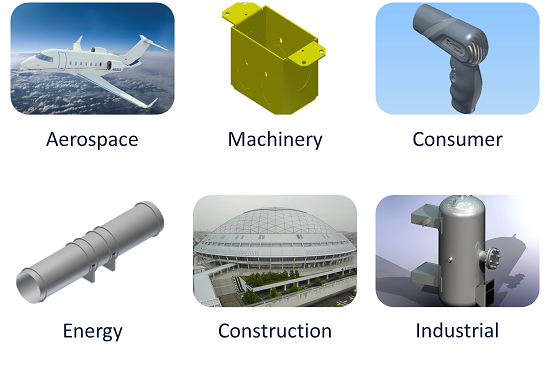
\includegraphics[width=0.6\linewidth]{../Common/images/ThinWallApplications.png}
			
		\end{center}
			
	\end{block}

	% ------------------------------------------------------------------------------------------------------------
			
	\begin{alertblock}{Problem Statement}
	
		\begin{center}
		
		{\Large ``Development of Algorithms for connected \textbf {Midsurface} mimicing 
		the original shape continuously, with no gaps, overlaps''}
		
		\bigskip
		
		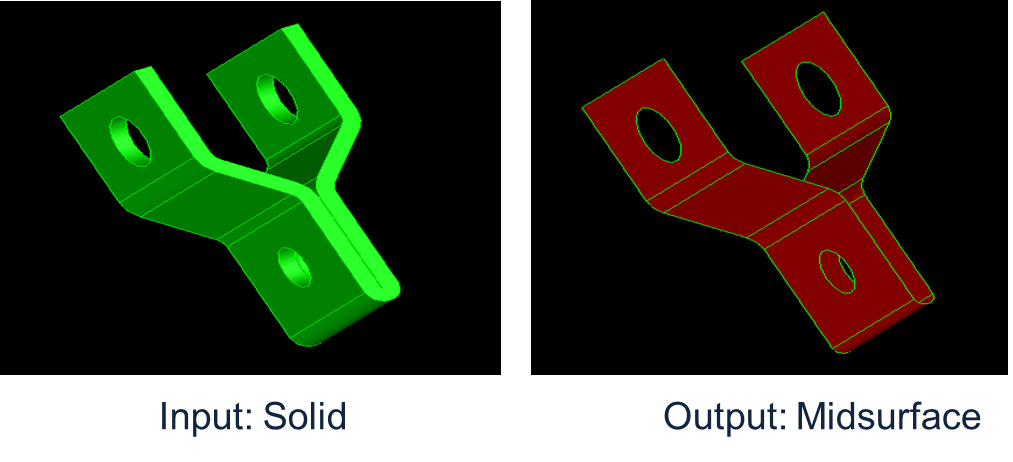
\includegraphics[width=0.9\linewidth]{../Common/images/SolidToMidsurface.png}
		
		\end{center}
		
	\end{alertblock}
	
		\begin{block}{Current Status}
	
		\begin{center}
		
			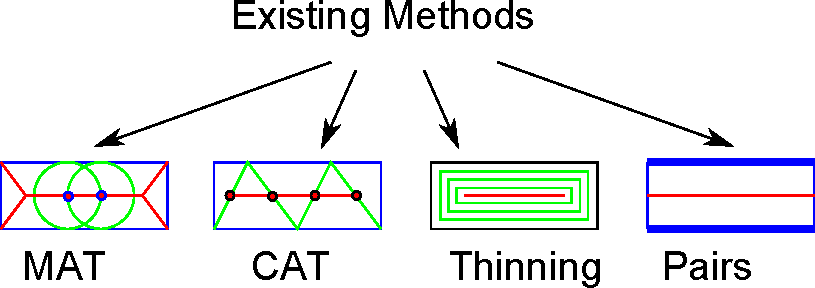
\includegraphics[width=0.9\linewidth]{../Common/images/MedialMethodsOnly.pdf}
		
			\vspace{2em}
			
			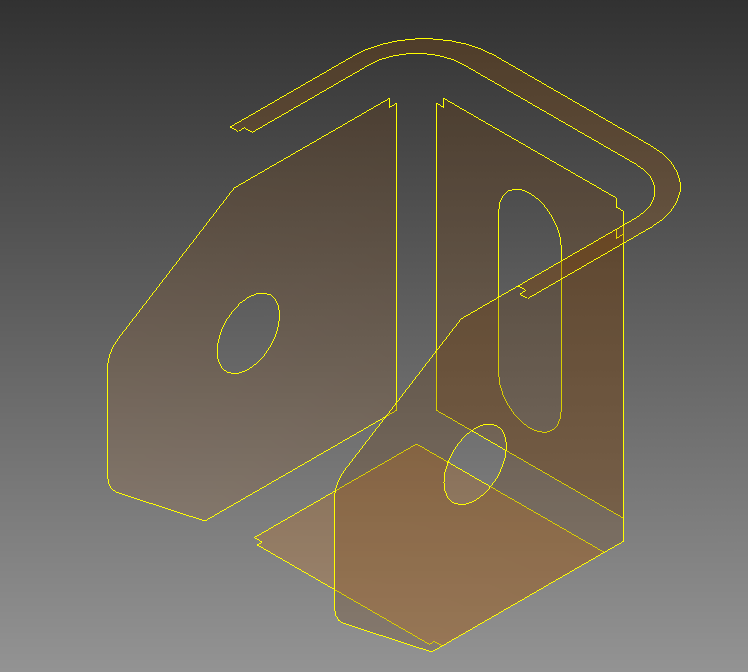
\includegraphics[width=0.65\linewidth]{../Common/images/Inventor_Bracket_MidsBorders.png}
			
		\end{center}
		
	\end{block}
		
			
\end{column}

%=================================================

\begin{column}{\onecolumnwidth} % The first column

		
		
	\begin{alertblock}{Divide-and-Rule}
		\begin{flushright}
			{\em Everything should be made as simple as possible, but not simpler \\- Albert Einstein}
		\end{flushright}
				
	\end{alertblock}
			
	\begin{block}{Leveraging Form Features}

		\centering 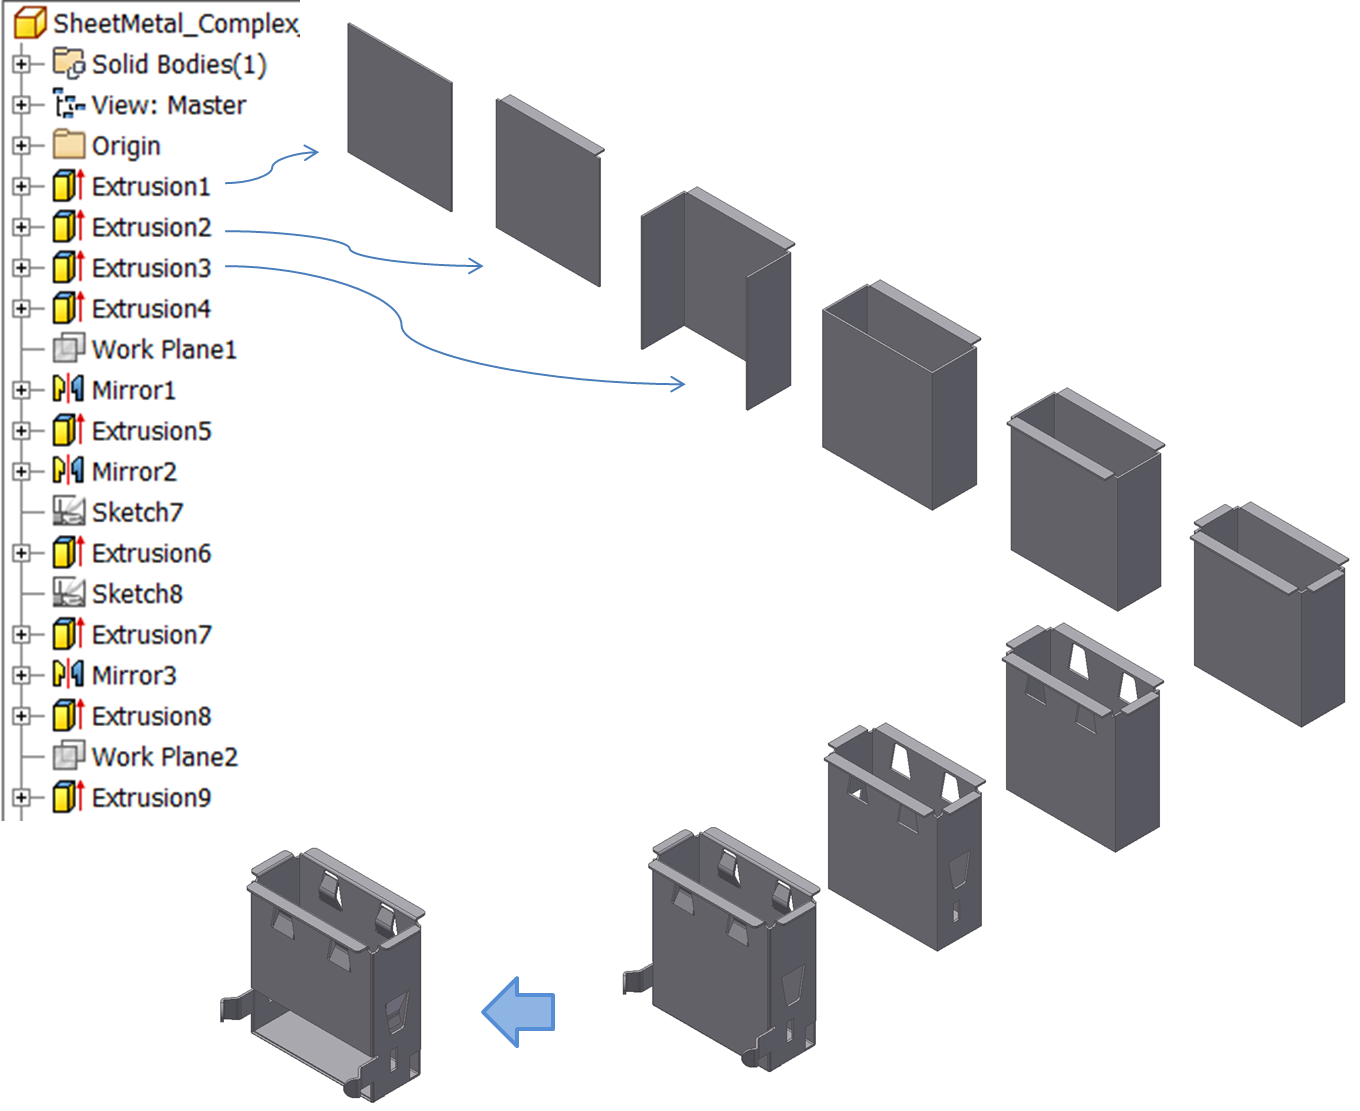
\includegraphics[height=0.65\linewidth]{../Common/images/USB_buildup}
	
	\end{block}

						
	\begin{block}{Proposed Idea}
	
	If this final shape is decomposed into smaller-simpler shapes, it would be easier and more deterministic to compute the midsurface. Such decomposition is readily available in the form of \textbf{features} and \textbf{cellular-decomposition}.
%	
%		\begin{itemize}
%		
%		\item To concurrently build mid-surfaces as part gets created 
%		\item At each feature step, shapes are relatively simple than final shape, 
%		\item Divide the feature volumes into Cells, build graph
%		\item Compute extensions at the interface nodes
%		
%		\end{itemize}
%		
%		\centering 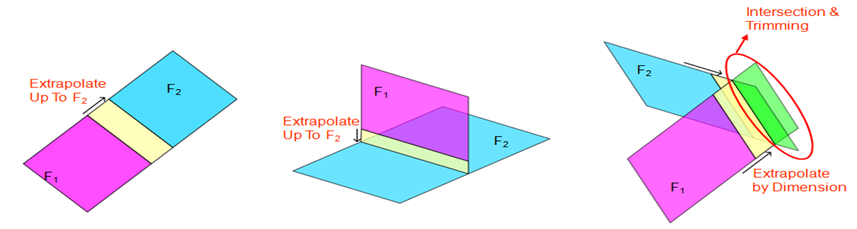
\includegraphics[width=0.9\linewidth]{../Common/images/ExtendTrim.png}
%		
	\end{block}


	\begin{block}{Workflow}
	
		\begin{center}
			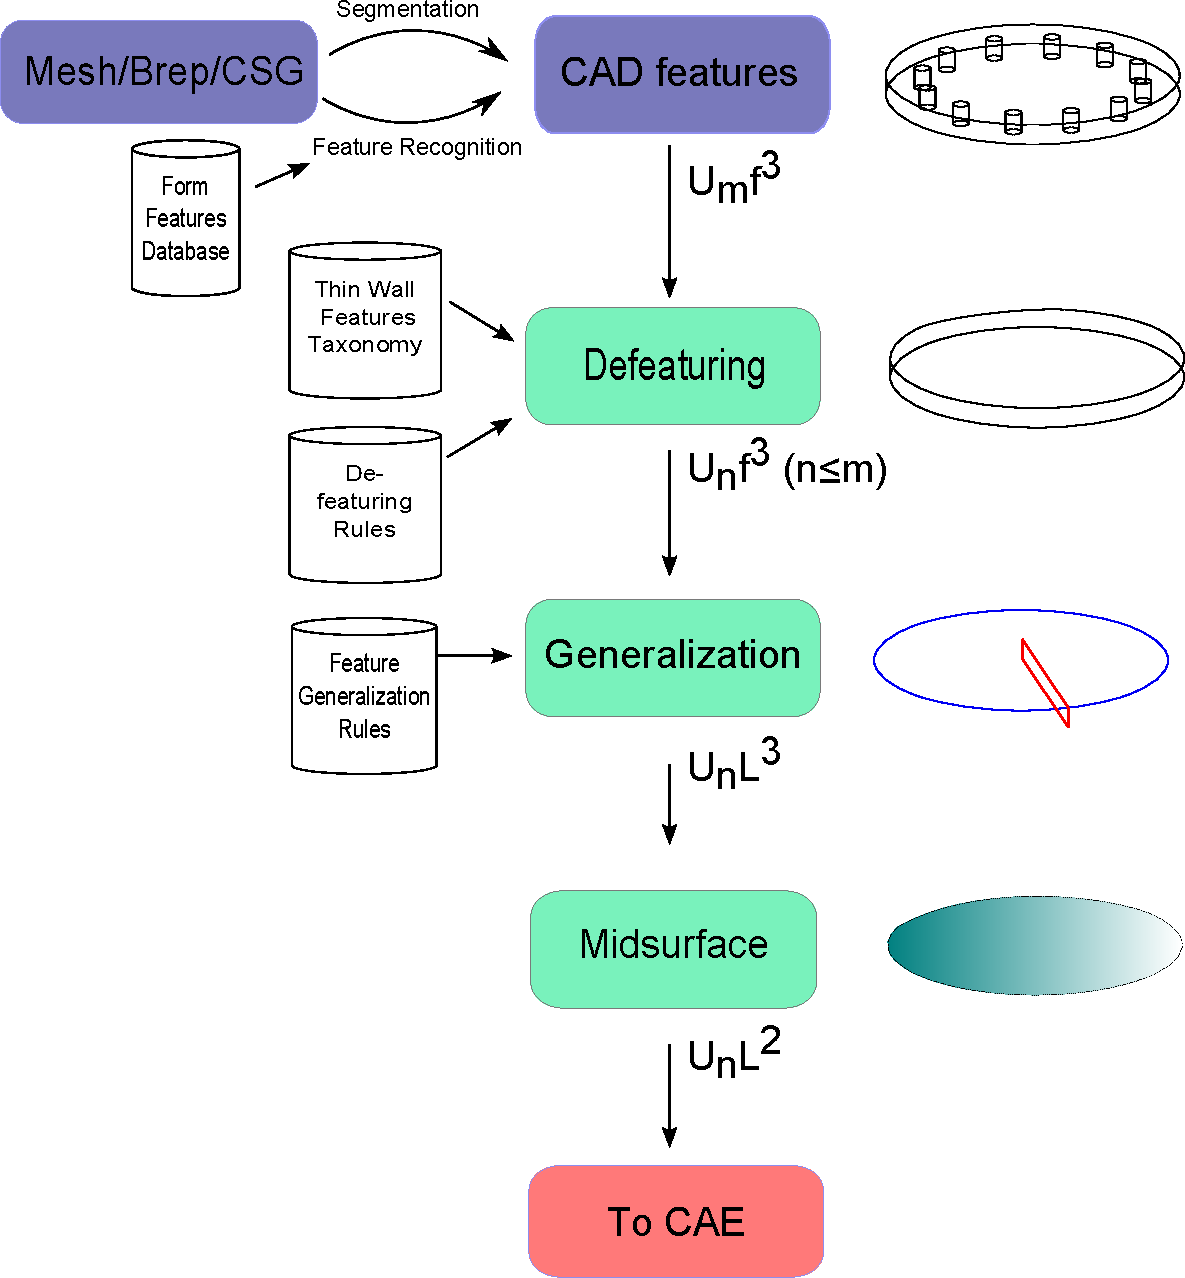
\includegraphics[width=0.9\linewidth]{../Common/images/SystemArchitecture2.pdf} 
		\end{center}
		
\vspace{0.5em}

\begin{itemize}[noitemsep,nolistsep]
		\item \textbf{Input}: Feature-based CAD model
		\item \textbf{Defeaturing}: Removes small features
		\item \textbf{Abstraction}: Transforms to generic Sweeps
		\item \textbf{Decomposition}: Forms cellular bodies' graph
		\item \textbf{Midsurface} Interfaces nodes connect midsurface patches created at the non-interface nodes.
\end{itemize}
		
	\end{block}
	

		
\end{column}

%===============================================

\begin{column}{\onecolumnwidth} % The first column

	\begin{block}{Midsurface}
		\begin{center}
			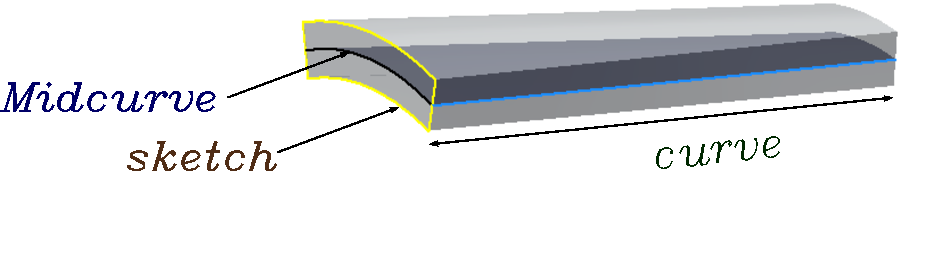
\includegraphics[width=0.9\linewidth]{../Common/images/MidsurfSmallProfile.pdf}
		\end{center}
		\vspace{-3.5em}
	\end{block}
	
	\begin{block}{Divide-and-Rule : 2D}
		\begin{tabular}{@{}p{0.3\linewidth}p{0.3\linewidth}p{0.3\linewidth}@{}}
			\raisebox{-0.9\height}{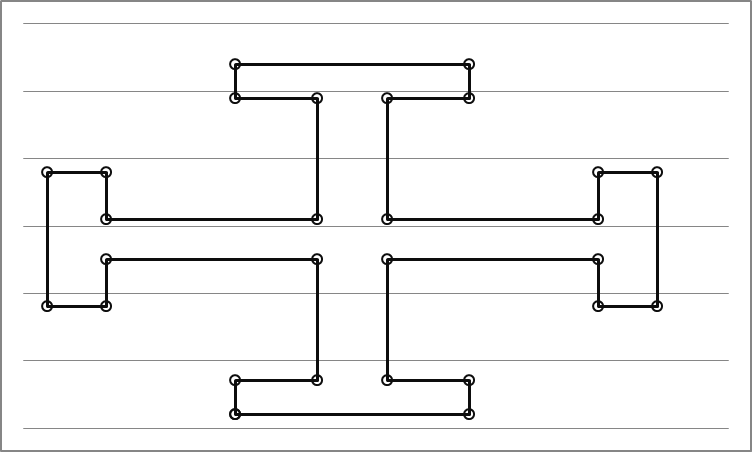
\includegraphics[width=0.9\linewidth]{../Common/images/Crosss}}
			&
			\raisebox{-0.9\height}{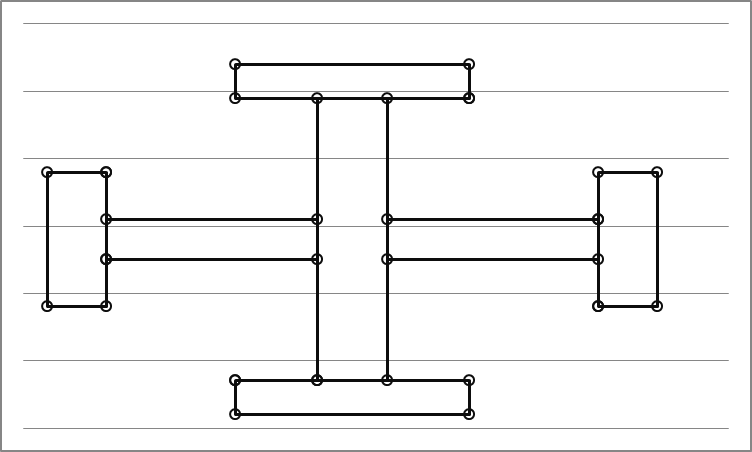
\includegraphics[width=0.9\linewidth]{../Common/images/Crossp}}
			&
			\raisebox{-0.9\height}{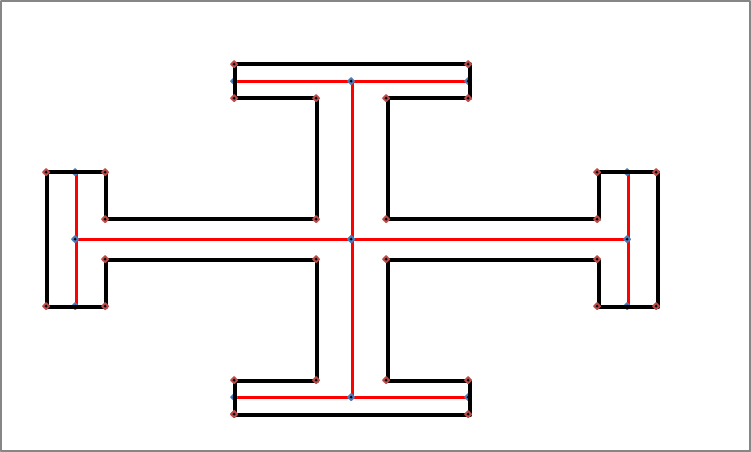
\includegraphics[width=0.9\linewidth]{../Common/images/Crossmc}}\\
		\end{tabular}
	\end{block}
	
	\begin{block}{Divide-and-Rule : 3D}
		\begin{center}
		\begin{tabular}[h]{@{}p{0.4\linewidth} p{0.4\linewidth} @{}} 
		
			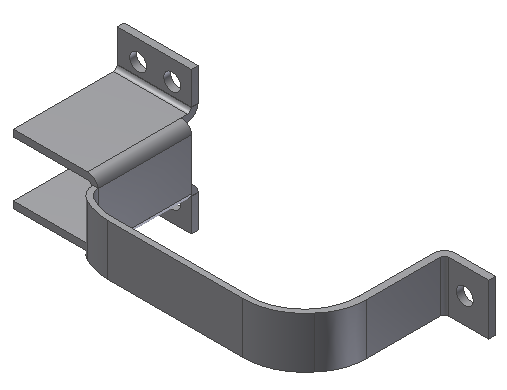
\includegraphics[width=0.8\linewidth]{../Common/images/nonCellularBracket}  &  
			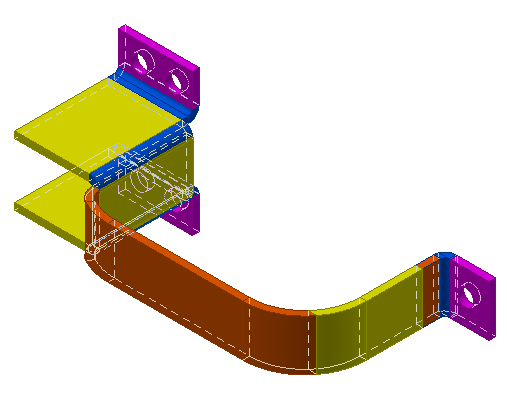
\includegraphics[width=0.8\linewidth]{../Common/images/CellularBracket}  \\
			
			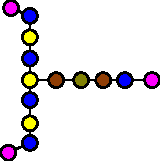
\includegraphics[width=0.8\linewidth]{../Common/images/CellGraphBracket.pdf} &  
			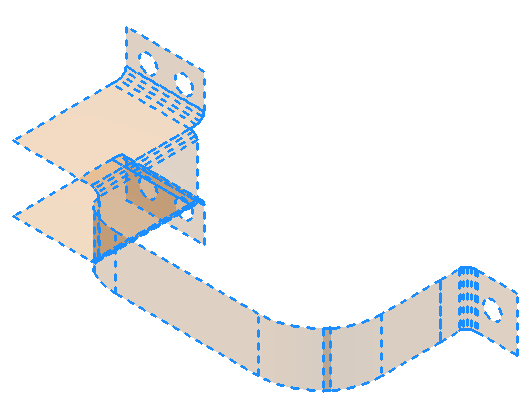
\includegraphics[width=0.8\linewidth]{../Common/images/midsCellularBracket} 	\\ 
			
		\end{tabular}	
		\end{center}
		\vspace{-1em}
	\end{block}
		
	\begin{block}{Advantages}
	
		\begin{itemize}
		
			\item Less manual rework, saving from hours to days
%			\item More and more thin-walled parts can be used from CAE analysis
%			\item Experimentation using changes in thickness gives flexibility
			\item Quicker design iterations and thus quicker time-to-market
			
		\end{itemize}
		
	\end{block}

%	\begin{block}{Conclusion}
%	
%		\begin{itemize}
%		
%			\item Features help in Model Simplification effectively, reducing resources-time 
%			\item Midsurface is concurrently built as part gets created at each feature level	
%			\item Abstraction represents neutral feature form helping portable algorithm
%			\item Cellular decomposition further divides for a uniform patch joining logic.
%			
%		\end{itemize}
%		
%	\end{block}

	\begin{alertblock}{Novelty}
	
		\begin{itemize}
		
			\item Use of a new Sheet Metal features Taxonomy for De-featuring
			\item Use remnant feature volumes for suppressibility
			\item Use of improved Polygon Decomposition and new Midcurves method
			\item New idea of Sweep based feature abstraction for portable algorithms
			\item Use of features for computation of Midsurface patches
			\item Use of Cells for generic connection logic for patches
			
		\end{itemize} 
		
	\end{alertblock}
		
	\begin{block}{Papers Published/Selected*}
	
		\begin{itemize}
		
			\item \textbf{Intl Conf, CoEP, 2013}: Feature Midsurface
			\item \textbf{Intl Conf, IITM, 2013}: Defeaturing
			\item \textbf{Intl Conf, IITG, 2014}:  Feature Abstraction
			\item \textbf{Intl Jrnl, Taylor \& Francis, 2015}
			\item \textbf{Intl Jrnl*/Conf, T \& F, London, 2015}
			\item \textbf{Intl Jrnl, Inderscience IJCAET, 2017*}
			
		\end{itemize} 
		
	\end{block}

	\begin{block}{References}

			\begin{itemize}
				\item \textbf{1967} Blum: Medial Axis Transform (MAT)
%				\item \textbf{1994} Dabke: Features for Idealization
				\item \textbf{1996} Armstrong: MAT for CAE
				\item \textbf{1996} Rezayat: Midsurface Abstraction
%				\item \textbf{2012} Russ: Features for De-featuring
				\item \textbf{2013} Woo: Cellular Decomposition, Midsurface
			
			\end{itemize} 	

	\end{block}

\end{column}

%================================================

\end{columns}
\end{frame}
\end{document}

